\subsection{Vorüberlegungen}
\label{bpr:vorueberlegungen}

Damit einige der Schritte im späteren Verlauf des Algorithmus im Bezug auf Indizes außerhalb des zu verarbeitenden Strings wohldefiniert sind, betrachten wir häufig eine erweiterte Version eines Strings gemäß Definition \ref{def:tplus}. Abbildung \ref{fig:tplus} zeigt beispielhaft eine Erweiterung eines Strings.

\begin{figure}[ht]
	\resizebox{\textwidth}{!}{
		\begin{tabular}{@{}l@{}}
			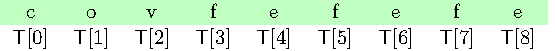
\includegraphics{kapitel/saca_algorithmen/bpr/algorithmus/phase1/t/image.pdf}\par\bigskip \\
			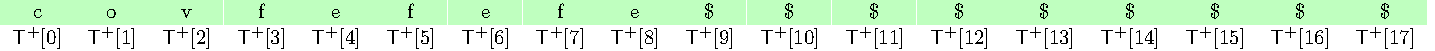
\includegraphics{kapitel/saca_algorithmen/bpr/algorithmus/phase1/tplus/image.pdf}
		\end{tabular}
	}
	\caption{Erweiterung von \inputtext zu \inputtextplus durch Anhängen von \(\$^n\)}
	\label{fig:tplus}
\end{figure}

\begin{definition}[\inputtextplus]
	\label{def:tplus}
    Sei \(\Sigma\) ein total geordnetes endliches Alphabet und \(\inputtext = \inputtext[0] \inputtext[1] \ldots \inputtext[n-1] \in \Sigma\) ein String über \(\Sigma\). Sei außerdem \(\$ \notin \Sigma\) ein nicht in \(\Sigma\) enthaltenes Symbol mit \(\forall c \in \Sigma : \$ < c\). Den um \(\$^n\) erweiterten String \(\inputtext\$^n\) nennen wir \inputtextplus.
\end{definition}

Ist das zugrunde liegende Alphabet außerdem total geordnet, so können auch die Suffixe eines Strings anhand dieser Ordnung sortiert werden.
Der Vergleich zweier Symbole des Alphabets bezüglich der Ordnung wird dadurch vereinfacht, dass jedem Symbol mit der Funktion \effective (Definition \ref{def:effective_alphabet}) eine natürliche Zahl als Rang zugewiesen wird.

Während für einzelne Symbole die Verwendung des effektiven Alphabets gegenüber dem direkten Vergleich keinen wesentlichen Vorteil erzielt, ergibt sich bei dem lexikographischen Vergleich zweier Strings bereits eine andere Situation: Auf Basis der Ränge der einzelnen Symbole kann auch ganzen Strings eine ganzzahlige Codierung zugewiesen werden, welche den Vergleich beschleunigt.

\begin{definition}[Stringkodierung]
	\label{def:coded}
	Sei \(\coded : (\Sigma \cup \{\$\})^d \rightarrow \{0, \ldots, (|\Sigma| + 1)^d - 1\}\) eine bijektive Funktion\footref{differs_from_paper}, sodass für zwei Strings \(u, v \in (\Sigma \cup \{\$\})^d\) gilt \(u < v \Leftrightarrow \coded(u) < \coded(v)\).
\end{definition}

Eine Stringkodierung wie in Definition \ref{def:coded} kann einfach unter Verwendung einer gegebenen \effective-Funktion (Definition \ref{def:effective_alphabet}) realisiert werden, indem die Symbole eines Strings abhängig von ihrem Index mit absteigender Wertigkeit für höhere Indizes summiert werden. Auf diese Weise ergibt sich für einen String \(\inputtext{[i,i+d)} = \inputtext[i] \ldots \inputtext[i + d - 1]\) die Kodierung \[\coded(\inputtext{[i,i+d)}) = \sum_{j=0}^{d - 1} (|\Sigma| + 1)^{d - 1 - j} \cdot \effective(\inputtext[i + j]).\]\par\smallskip
Auch Kodierungen für Strings größerer Länge als \(d\) können auf diese Weise berechnet werden, indem alle Symbole an Indizes größer oder gleich \(d\) ignoriert werden. Aufgrund der hier gewählten Berechnungsvorschrift für \coded lassen sich außerdem auf sehr einfache Weise Kodierungen für aufeinanderfolgende Suffixe berechnen.
\begin{equation}
	\label{eq:coded}
    \coded(\suffix{i+1}) = (|\Sigma| + 1) \cdot \left( \coded(\suffix{i}) \text{ mod } (|\Sigma| + 1)^{d-1}\right) + \effective(\inputtextplus[i+d])
\end{equation}
Man beachte hier, dass für zwei aufeinanderfolgende Suffixe \suffix{i} und \suffix{i+1} lediglich das erste Symbol aus \suffix{i} aus der Kodierung entfernt werden muss (mittels mod \((|\Sigma| + 1)^{d-1}\)), woraufhin die Wertigkeit aller verbleibenden Symbole jeweils um eine Stelle ansteigt. Zuletzt muss nur noch der Rang des letzten Symbols aus \suffix{i+1} hinzu addiert werden.\par\smallskip
Wie viele andere Algorithmen zur Konstruktion von Suffix-Arrays, arbeitet auch \bpr mit einer Unterteilung des Suffix-Arrays in sogenannte Buckets (Definition \ref{def:bucket} auf Seite \pageref{def:bucket}). Die Unterteilung des Arrays in Buckets ist erforderlich, um das Suffix-Array schrittweise sortieren zu können, indem bestehende Buckets durch Aufteilung weiter verfeinert werden.
